\chapter{Systemdesign og implementasjon}
\label{chap:system}

\section{Krav og designmål}
\label{sec:krav-designmal}
Gjennom internship PRA400- 2025 jobbet jeg med å designe appen i prototype og figma for å ha en klar design som kan bygge appen på. 
Applikasjonen er utviklet for å støtte en strukturert registreringsflyt der brukeren kan samle inn bilde(r) og tilhørende metadata for videre behandling. Et sentralt krav var at løsningen skulle fungere på tvers av plattformer, samtidig som arbeidsflyten skulle være enkel å forstå for brukere med varierende digital kompetanse \cite{stellai_projectdoc_2025}.

Designmålene ble formulert med vekt på:
\begin{itemize}
  \item \textbf{MVP-fokus:} identifisere og implementere kjerneoppgavene først for raskt å etablere en testbar ende-til-ende flyt.
  \item \textbf{Lav friksjon i navigasjon:} redusere antall steg og gjøre skjermoverganger forutsigbare.
  \item \textbf{Strukturert registrering:} sikre at bilder, kategori og metadata blir samlet i én sammenhengende registrering som kan sendes videre.
\end{itemize}

\section{Arkitektur (frontend / backend)}
\label{sec:arkitektur}
\textbf{Frontend.} Applikasjonen er implementert med Expo og React Native, som muliggjør en felles kodebase og rask iterasjon på mobilfunksjonalitet.

\textbf{Backend (fase 1 -- Firebase).} I en tidlig fase ble Firebase valgt for autentisering og lagring for å etablere en fungerende ende-til-ende flyt raskt.

\textbf{Backend (fase 2 -- Azure).} I videreutviklingen av masterprosjektet er løsningen flyttet til Azure, da det samsvarer med valgt skyplattform i målmiljøet og forenkler videre utvikling og integrasjon. I nåværende løsning sendes bilde og metadata til lagring i Azure, med Microsoft-basert innlogging.

\section{Håndtering av systemtilstand}
\label{sec:systemtilstand}
Applikasjonen er bygget rundt en registrering som består av (1) bilde(r), (2) kategori/avfallstype og (3) metadata (for eksempel kundenummer og kjøreordre), etterfulgt av (4) innsending til skylagring. Dette krever robust håndtering av systemtilstand gjennom flere skjermoverganger.

I masteroppgaven forstås systemtilstand særlig gjennom:
\begin{itemize}
  \item \textbf{Persistens av metadata:} informasjon skrevet inn før bilde tas/velges må bevares ved navigasjon til kamera og tilbake.
  \item \textbf{Kobling mellom bilder og aktiv registrering:} bilder skal tilhøre én aktiv registrering og ikke blandes med tidligere innsendinger.
  \item \textbf{Tydelig sluttpunkt:} etter innsending skal det være entydig at registreringen er fullført og at systemet er klar for neste.
\end{itemize}

\section{Lokal lagring (AsyncStorage)}
\label{sec:asyncstorage}
For å støtte flertrinns arbeidsflyt benyttes lokal lagring (AsyncStorage) til å persistere utkast-/sesjonsdata midlertidig. Dette er relevant for å redusere risiko for datatap i overganger mellom skjermbilder og for å kunne gjenoppta en registrering uten å starte på nytt.

Lokal lagring er samtidig et sentralt evalueringspunkt i masteren: løsningen må bevare nødvendig informasjon når det er forventet, men også tømmes korrekt for å unngå gjenbruk av tidligere data i nye registreringer.

\section{Reset-logikk}
\label{sec:reset}
Etter vellykket innsending skal systemet starte neste registrering i tom tilstand. Reset-logikken skal derfor:
\begin{itemize}
  \item tømme bildeliste og tilhørende metadata,
  \item tømme relevant lokal lagring knyttet til forrige registrering,
  \item sikre at brukergrensesnittet fremstår klart til neste innsending.
\end{itemize}

I dagens løsning er følgende utfordringer identifisert og danner grunnlag for evalueringen:
\begin{itemize}
  \item metadata kan forsvinne ved skjermbytte (indikasjon på mangelfull persistens),
  \item tidligere sendte bilder kan vises ved ny registrering (indikasjon på mangelfull reset av state og/eller lokal lagring).
\end{itemize}

\section{Identifiserte tekniske utfordringer}
\label{sec:tekniske-utfordringer}
Dokumentasjonen beskriver implementerte kjernefunksjoner som autentisering, bildeopptak/opplasting, profilfunksjoner og validering før innsending \cite{stellai_projectdoc_2025}. Videre er det beskrevet at feil- og nettverkshåndtering er viktig for stabilitet i brukerflyt, samt at prosjektet ble strukturert med versjonskontroll for sporbarhet og vedlikehold \cite{stellai_projectdoc_2025}.
\newline
Her er tenlogivalgene som ble brukt i prosjektet under utvikling: Det ble React Native me Expo til frontend utvikling og samme me Firebase og Azure til authction og skyplattform. 

\subsection{Valg av React Native fremfor Flutter og andre rammeverk}
Når det gjelder mobilapplikajson, så er det mest konsekvensrike beslutningene er å valge av et cross-plattform rammeverk. I Stellai master prosjektet React Native og Flutter var de mest konkurrentene til mobilapplikasjonen, så etter flere team mter og undersøkelser landet jeg på React Native me Expo til frontend utvikling. 

\subsubsection{Bakgrunn:} Kompetansen og kunnskap i TypeScript tatt med i vurdering av rammeverk-tknologi. React Native benytter typeScript som programmeringsspråk og det programmeringsspråketet er bruket av 62,3\% av utviklere på verdensbasis\cite{stackoverflow_dev_survey_2024_technology}

\begin{figure}[H]
    \centering
    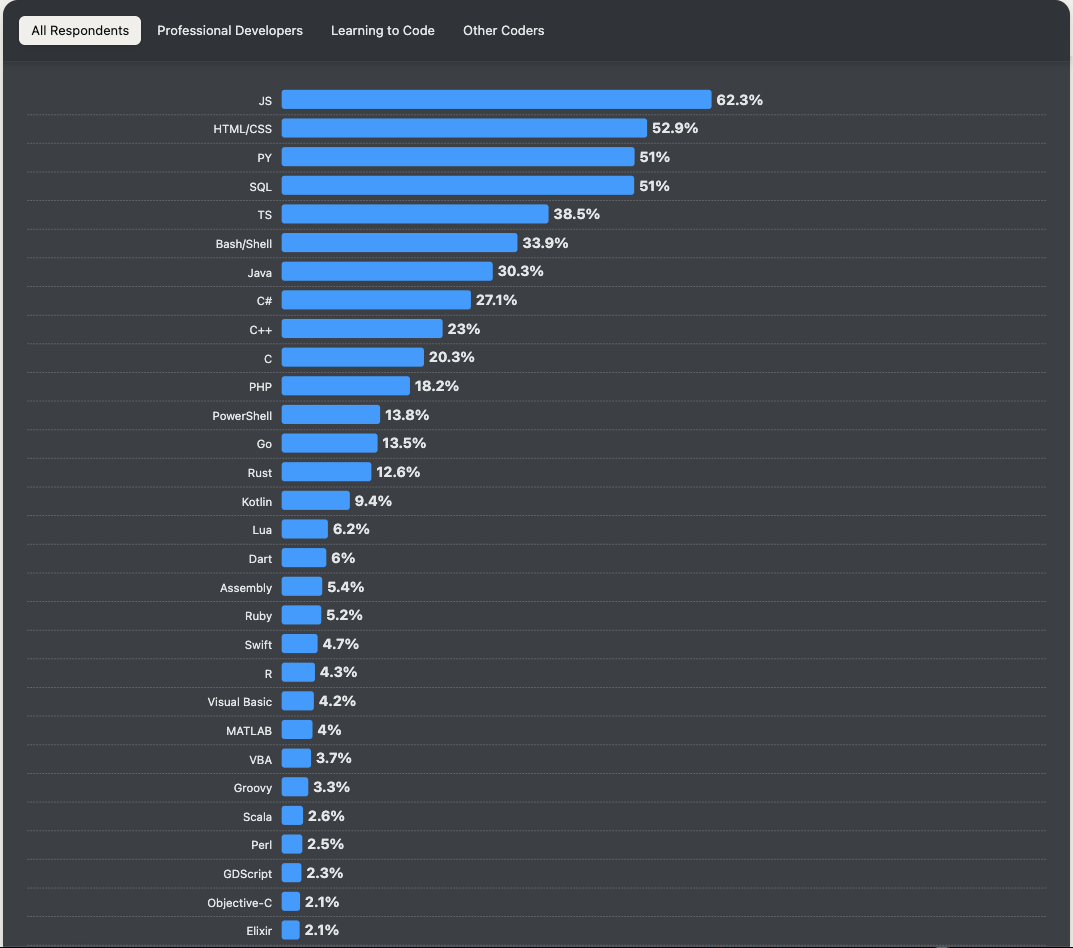
\includegraphics[width=0.8\textwidth]{Figures/Typescript.png}
    \caption{Det mest populære programmeringsspråket.\cite{stackoverflow_dev_survey_2024_technology}}
    \label{fig:mittbilde}
\end{figure}


\subsubsection{Flutter(Dart):} Dart er eneste språket du bruker for å skrive selve Flutter-appen, noe som krever ny innlæring av nytt programmeringsspråk. I denne masteroppgaven med tidsbegrensing og fokos p funksjonalitet og brukertesting er Dart ikke så smart valg spesilet kreves ny innlæring.

\subsubsection{Expo:} Tidlgere erfaring me React Native og Expo har gjort at Expo ble valgt som ramme for applikasjonsbygging. Expo gjør setup mye raskere og enklere, den gir utvikler rask hot-reloaf. Expo tilbyr også en ferdig implementerte API‑er for kamerahåndtering, filsystemoperasjoner og vedvarende lokal lagring via AsyncStorage. Dette reduserer arbeidstid og komme raskt i gang me utviklg. 

\subsection{Bruk av Firebase i prosjektet} I starten av utviklingsprosessen ble Firebase valgt som backend. Firebase er en Backend-as-a-Service (BaaS)-løsning fra google, og den gir ferdigkonfigurerte backend-tjenester som autentisering. Ingen serveroppsett, plug-and-play-autentisering dette reduserer tid for å komme raskt i gang me MVP. 

\subsection{Bruk av azure:} Stellai bruker azure for kundne sine for register og log in via Microsoft tjensten og derfor er det anbefalt av tekniske sjef om bruk av azure til Auth og Storage. 



\begin{table}[h]
\label{tab:teknologivalg}

\renewcommand{\arraystretch}{1.3}

\begin{tabularx}{\textwidth}{|>{\raggedright\arraybackslash}p{4.1cm}
                            |>{\raggedright\arraybackslash}X
                            |>{\raggedright\arraybackslash}X|}

\hline
\rowcolor{uialightgold}
\textbf{Vurdering} & 
\textbf{Fordel} & 
\textbf{Ulemp} \\
\hline
React Native VS Flutter&
React Native: TypeScript (javaScript) som er kjent og bruk av 62,3\% av utviklere i Web og app utvikling. &
Flutte: Dart som hoved Programmeringsspråk og kreves nytt innlæring \\
\hline
Firebase og azure &
BaaS/MBaaS kan redusere oppstartskost ved å tilby ferdige backend-tjenester; ofte egnet i tidlige prototyper. Stellai bruker Azure og derfor er det sterkt ble valgt.&
Firebase er primært rettet mot startups og småprosjekter og prismodell bli uforholdsmessig dyr sammenlignet med infrastrukturtjenester (IaaS) som Azure.\\
\hline
\end{tabularx}


\caption{Teknologivalg i systemet}
\label{tab:teknologivalg}
\end{table}




